% hdp
\lecture{The Hierarchical Dirichlet Process}{hdp}

\begin{frame}
	\frametitle{The Hierarchical DP}
	\begin{itemize}
		\item Imagine we have $>1$ related dataset to cluster, generated by the same process
		\item Fitting separate mixtures to each results in a loss of information
		\item The \ac{HDP} allows them to be analysed together with shared parameters
		\begin{itemize}
			\item e.g. datasets clustered individually but cluster parameters (e.g. means) can be \emph{shared}
			\item Analogy: The Chinese Restaurant Franchise
			\item Described in \href{http://www.cs.berkeley.edu/~jordan/papers/hdp.pdf}{Teh et.~al}
		\end{itemize}
	\end{itemize}
\end{frame}

\begin{frame}
	\frametitle{The Chinese Restaurant Franchise}
	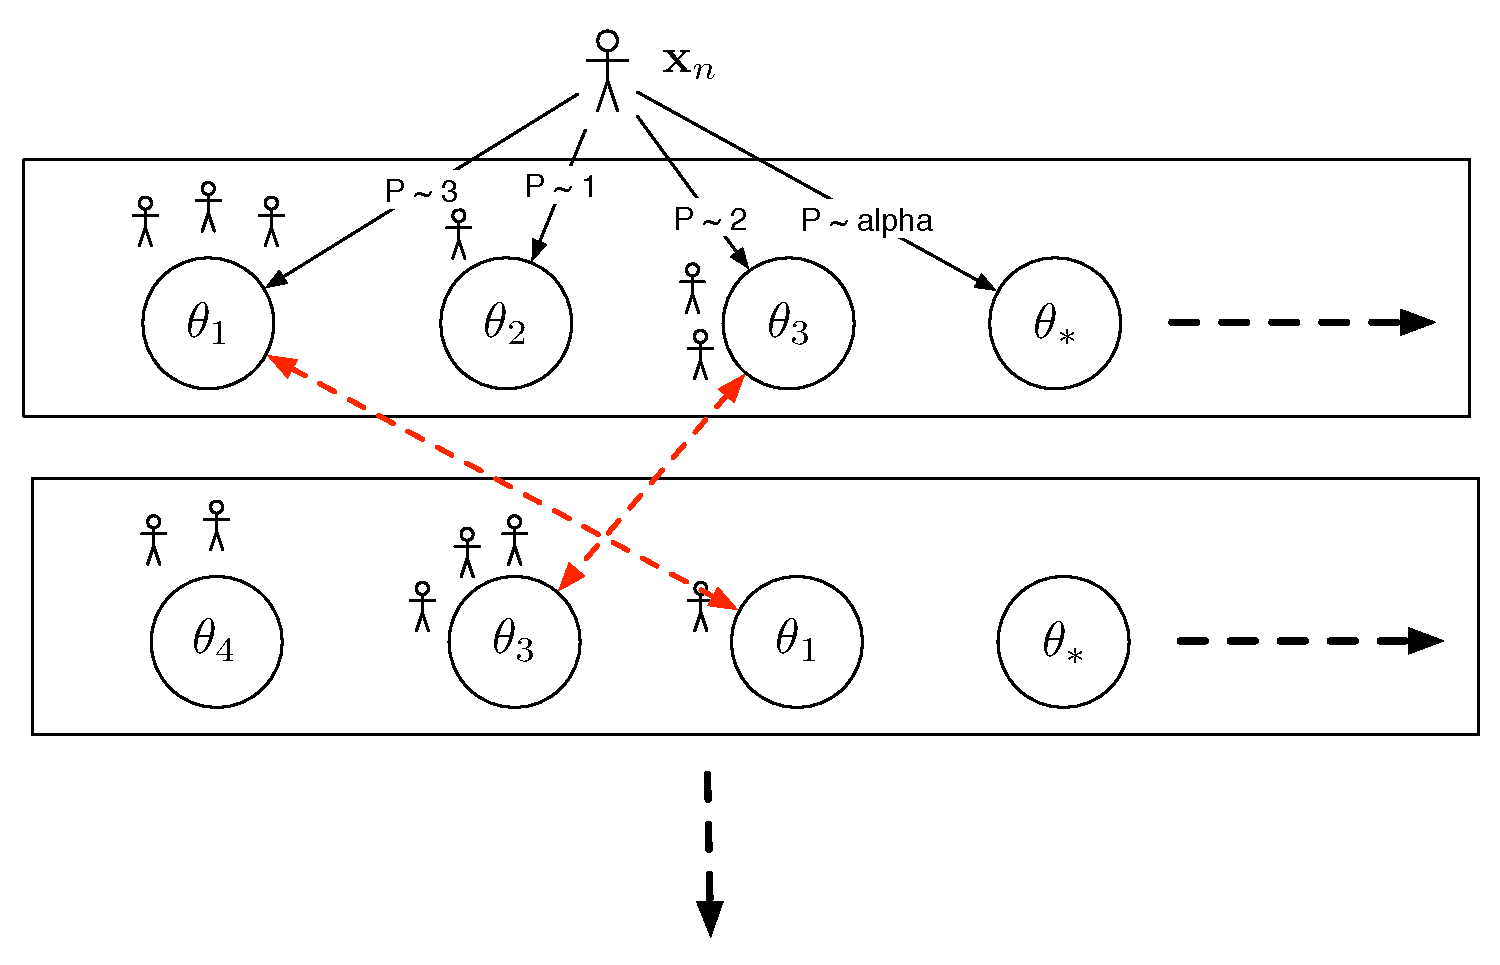
\includegraphics[width=\linewidth]{CRPfranchise}
\end{frame}

\begin{frame}
	\frametitle{The Chinese Restaurant Franchise}
	\begin{itemize}
		\item Gibbs sampling is very similar to the single restaurant case
		\item Each object is re-assigned to a table with probabilities ($i$ indexes datasets):
		\[
			P(z_{ink} = 1|\ldots)\propto \left\{
			\begin{array}{cc}
				n_{ik}p(\bx_{in}|\theta_k) & \mbox{for current table}\\
				\alpha p(\bx_{in}) & \mbox{for new $k$}
			\end{array}
			\right.			
		\]
		\item $p(\bx_{in})$ is computed by marginalising all possible values for the parameters at the new tables.
		\begin{itemize}
			\item These include values used for current tables (with prior proportional to the number of tables they're used at) and a completely new value (with prior proportional to, say, $\gamma$).
			\item i.e. There are \ac{DP}s for assignment of objects to tables and assignment tables to parameters.
		\end{itemize}
	\end{itemize}
\end{frame}

\begin{frame}
	\frametitle{Data sampled from a \ac{HDP}}
	\begin{multicols}{2}
		\centering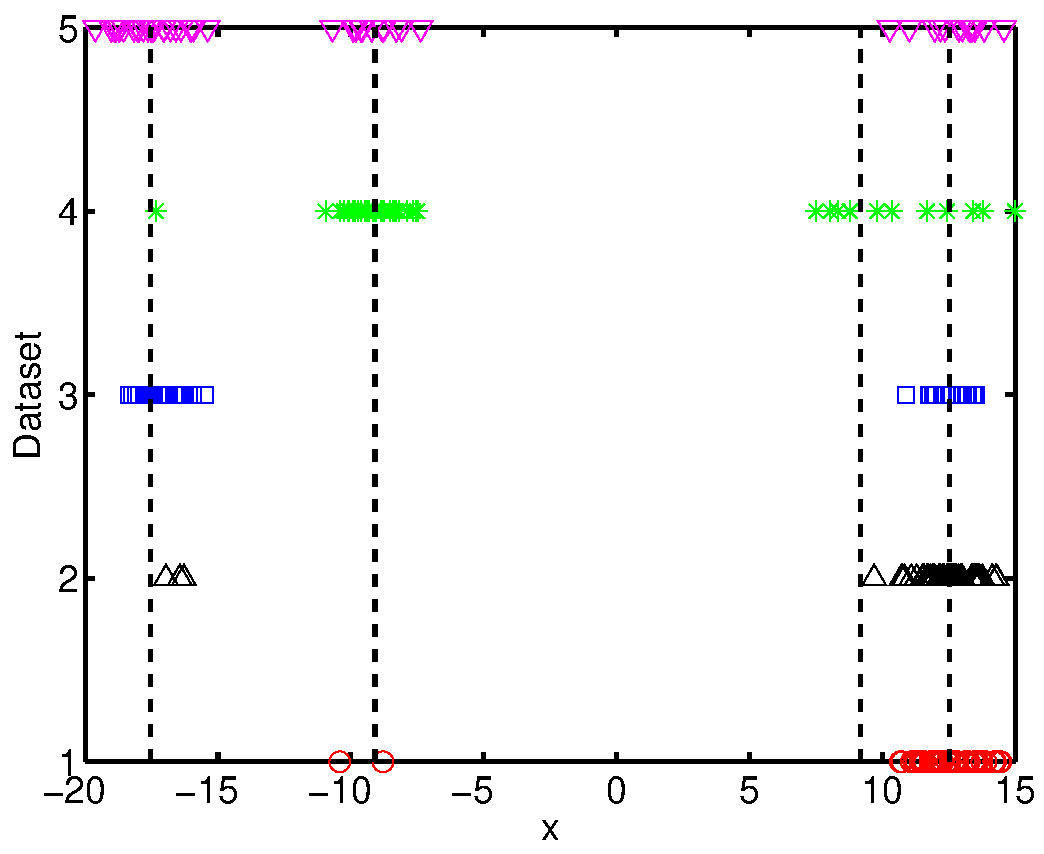
\includegraphics[width=\linewidth]{hdp_data}
		\newpage
		\begin{itemize}
			\item 5 datasets
			\item 4 top level components (dashed line)
			\item Each data has data from a subset of components
		\end{itemize}
	\end{multicols}
\end{frame}

\begin{frame}
	\frametitle{\ac{HDP} inference example}
	\begin{multicols}{2}
	\begin{itemize}
		\item 300 posterior samples.
		\item Does pretty good job.
		\item At last sample, posterior means over top-level components were: 12.5215, -17.0304, -9.0535, 8.7857, -17.5636, -16.12
		\item True: [12.5185,-9.0909,-17.5295,9.1839]
	\end{itemize}
	\newpage
	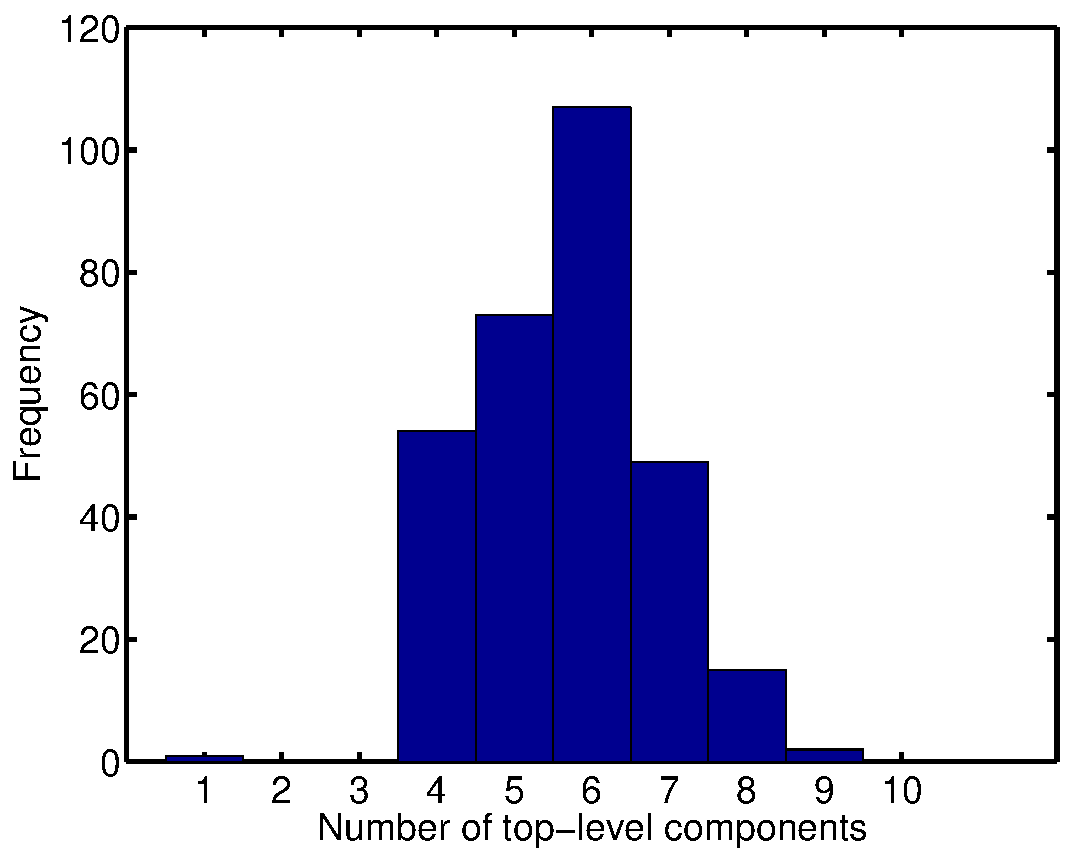
\includegraphics[width=\linewidth]{hdp_inference}		
	\end{multicols}
	\begin{itemize}
		\item Note that mixing would be improved by also re-sampling assignment of clusters to top components.
	\end{itemize}
\end{frame}